\documentclass[aspectratio=169]{beamer}
\usetheme{Madrid}
\usecolortheme{default}

\usepackage[utf8]{inputenc}
\usepackage{amsmath}
\usepackage{graphicx}
\usepackage{booktabs}
\usepackage{xeCJK}

\title{ECE489 中期答辩}
\subtitle{四足机器人运动控制：\\强化学习与模型预测控制}
\author{Shihong Yuan (3230116076), Junxiao Wang (3230112131)}
\institute{University of Waterloo}
\date{2026年5月14日}

\begin{document}

\frame{\titlepage}

% Slide 1: 项目概述
\begin{frame}{项目概述与目标}
\begin{block}{项目目标}
开发四足机器人（Unitree Go2）的运动控制器，实现平地和斜坡地形的稳定行走
\end{block}

\begin{columns}[T]
\column{0.5\textwidth}
\textbf{实现方法：}
\begin{itemize}
    \item \textbf{方法A：}强化学习（PPO算法）
    \item \textbf{方法B：}模型预测控制（MPC）
    \item 对比两种方法的性能
\end{itemize}

\column{0.5\textwidth}
\textbf{评估指标：}
\begin{itemize}
    \item 速度跟踪精度
    \item 身体稳定性
    \item 能量效率（CoT）
    \item 抗干扰能力
\end{itemize}
\end{columns}

\vspace{0.3cm}
\begin{center}
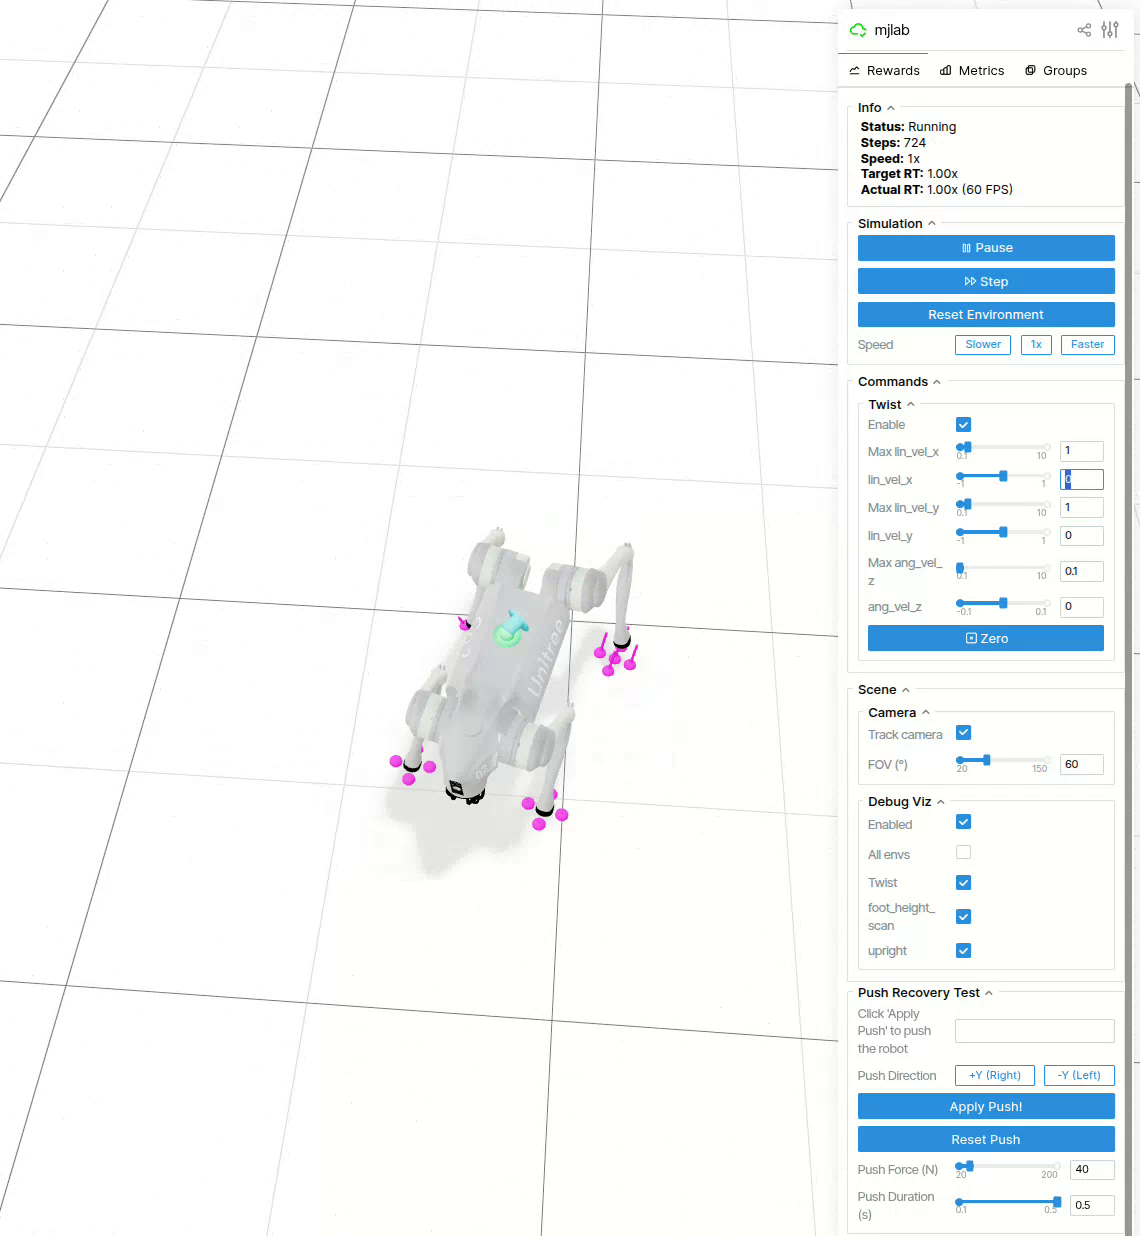
\includegraphics[width=0.6\textwidth]{rl_flat_1.png}
\end{center}
\end{frame}

% Slide 2: 仿真环境设置
\begin{frame}{仿真环境设置}
\begin{columns}[T]
\column{0.5\textwidth}
\textbf{仿真平台：mjlab + MuJoCo}
\begin{itemize}
    \item GPU加速的并行仿真
    \item 高保真接触动力学
    \item 机器人：Unitree Go2（12自由度）
\end{itemize}

\vspace{0.3cm}
\textbf{训练配置：}
\begin{itemize}
    \item 平地：2048个并行环境
    \item 斜坡：512个并行环境
    \item 控制频率：50 Hz
    \item Episode长度：20秒
\end{itemize}

\column{0.5\textwidth}
\textbf{地形类型：}
\begin{itemize}
    \item \textbf{平地：}均匀摩擦系数
    \item \textbf{斜坡：}5-55度倾斜
\end{itemize}

\vspace{0.3cm}
\begin{center}
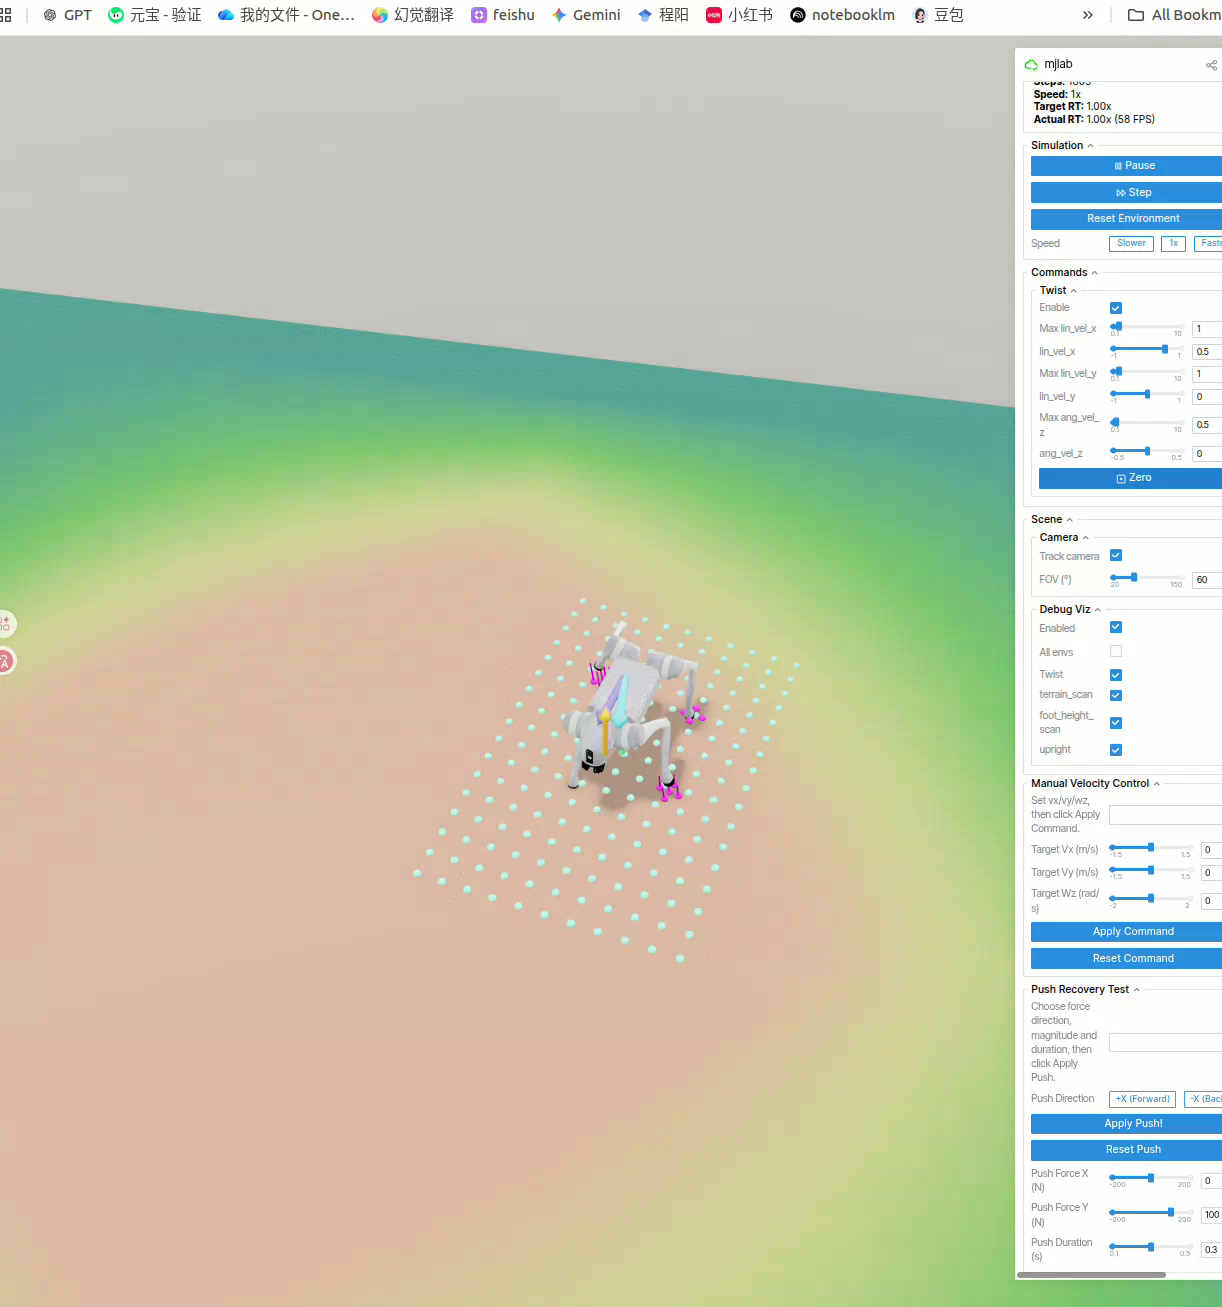
\includegraphics[width=\textwidth]{rl_slope_1.png}
\end{center}
\end{columns}
\end{frame}

% Slide 3: 强化学习方法
\begin{frame}{强化学习方法：PPO算法}
\begin{columns}[T]
\column{0.55\textwidth}
\textbf{PPO目标函数：}
\begin{equation*}
L^{CLIP}(\theta) = \mathbb{E}_t\left[\min\left(r_t(\theta)\hat{A}_t, \text{clip}(r_t(\theta), 1-\epsilon, 1+\epsilon)\hat{A}_t\right)\right]
\end{equation*}

\textbf{观测空间（平地）：}48维
\begin{itemize}
    \item 身体线速度/角速度（6维）
    \item 投影重力（3维）
    \item 关节位置/速度（24维）
    \item 历史动作（12维）
    \item 速度指令（3维）
\end{itemize}

\textbf{动作空间：}12维
\begin{itemize}
    \item 期望关节位置（PD控制器输入）
\end{itemize}

\column{0.45\textwidth}
\textbf{奖励函数设计：}
\begin{itemize}
    \item \textbf{速度跟踪}（权重3.0）
    \begin{equation*}
    \small r_{lin} = 3.0 \cdot e^{-\frac{\|v_{cmd} - v_{actual}\|^2}{0.15}}
    \end{equation*}

    \item \textbf{直立姿态}（权重0.5）
    \item \textbf{平滑运动}（权重-0.05）
    \item \textbf{足部离地高度}（权重-0.75）
    \item \textbf{步态时序}（权重0.25）
\end{itemize}

\vspace{0.2cm}
\textbf{域随机化：}
\begin{itemize}
    \item 摩擦系数：$\mu \in [0.5, 1.2]$
    \item 质量：$\pm 20\%$
    \item 电机强度：$\pm 10\%$
\end{itemize}
\end{columns}
\end{frame}

% Slide 4: 初步训练结果
\begin{frame}{初步训练结果}
\begin{columns}[T]
\column{0.5\textwidth}
\textbf{平地训练（500次迭代）}
\begin{center}
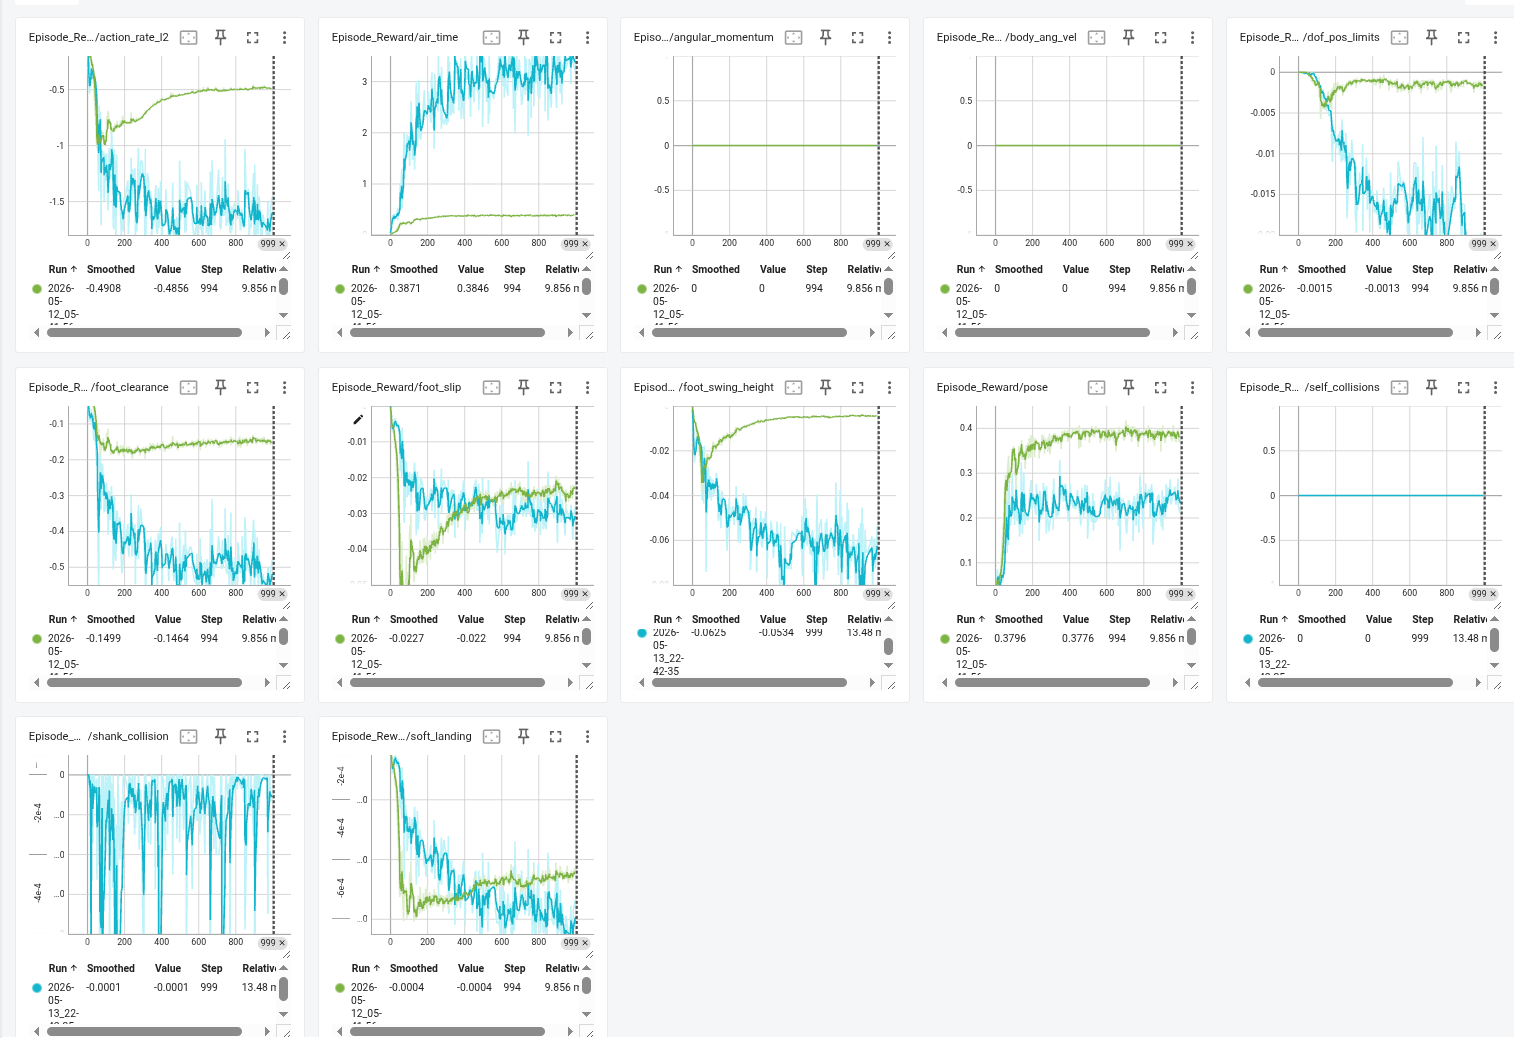
\includegraphics[width=\textwidth]{flat_slope1.png}
\end{center}

\textbf{观察：}
\begin{itemize}
    \item 约300次迭代后收敛
    \item 最终奖励 $\sim$ 8.5
    \item 训练时间：2-3小时
\end{itemize}

\column{0.5\textwidth}
\textbf{斜坡训练（1000次迭代）}
\begin{center}
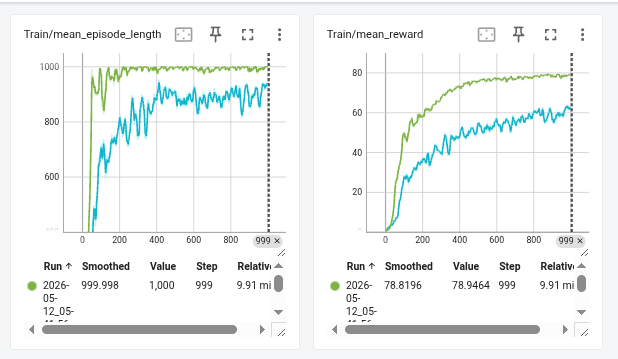
\includegraphics[width=\textwidth]{flat_slope2.png}
\end{center}

\textbf{观察：}
\begin{itemize}
    \item 约600次迭代后收敛
    \item 最终奖励 $\sim$ 7.2
    \item 训练时间：4-5小时
    \item 方差更大（地形复杂）
\end{itemize}
\end{columns}
\end{frame}

% Slide 5: 域随机化的重要性
\begin{frame}{关键发现：域随机化的必要性}
\begin{center}
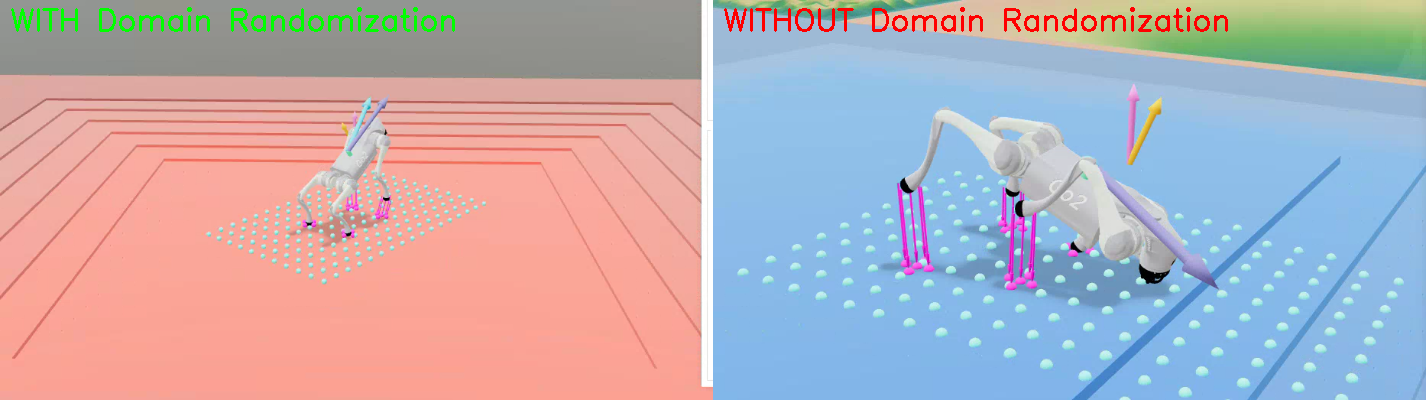
\includegraphics[width=0.9\textwidth]{dr_comparison.png}
\end{center}

\begin{block}{重要发现}
\textbf{没有域随机化，策略完全无法学习运动！}机器人要么静止不动，要么立即摔倒。
\end{block}

\textbf{原因分析：}
\begin{itemize}
    \item 防止过拟合到标称参数（摩擦=1.0，标称质量）
    \item 强制策略发现在多种条件下都有效的鲁棒策略
    \item 为sim-to-real迁移做准备（真实世界参数永远不会完全匹配仿真）
\end{itemize}
\end{frame}

% Slide 6: 初步性能评估
\begin{frame}{初步性能评估}
\begin{table}
\centering
\caption{RL控制器初步性能（平地，前向运动1.0 m/s）}
\small
\begin{tabular}{lcc}
\toprule
\textbf{指标} & \textbf{结果} & \textbf{目标} \\
\midrule
前向速度 $v_x$ & 0.963 $\pm$ 0.090 m/s & 1.0 m/s \\
横向速度 $v_y$ & -0.003 $\pm$ 0.042 m/s & 0 m/s \\
Roll标准差 & 2.50° & < 5° \\
Pitch标准差 & 0.82° & < 5° \\
能量效率（CoT） & 133.13 & < 100 \\
抗推力恢复率 & 40.0\% & > 80\% \\
\bottomrule
\end{tabular}
\end{table}

\vspace{0.3cm}
\begin{columns}[T]
\column{0.5\textwidth}
\textbf{优势：}
\begin{itemize}
    \item 前向速度跟踪良好（96.3\%）
    \item 姿态稳定性可接受
\end{itemize}

\column{0.5\textwidth}
\textbf{待改进：}
\begin{itemize}
    \item 能量效率偏低
    \item 抗干扰能力不足
    \item 横向运动待测试
\end{itemize}
\end{columns}
\end{frame}

% Slide 7: 遇到的困难与解决方案
\begin{frame}{遇到的困难与解决方案}
\begin{block}{困难1：训练不稳定}
\textbf{问题：}初期训练奖励波动大，策略不收敛\\
\textbf{解决：}引入域随机化，调整奖励函数权重，增加并行环境数
\end{block}

\begin{block}{困难2：横向运动性能差}
\textbf{问题：}横向速度跟踪精度低（84.1\%），抗推力恢复率0\%\\
\textbf{计划：}增加横向运动的奖励权重，延长训练时间，引入显式干扰训练
\end{block}

\begin{block}{困难3：能量效率低}
\textbf{问题：}CoT值偏高（133 vs 目标<100）\\
\textbf{计划：}增加平滑运动的惩罚权重，优化步态模式
\end{block}

\begin{block}{困难4：观测空间维度高}
\textbf{问题：}斜坡地形需要187维高度扫描，导致训练变慢\\
\textbf{解决：}减少并行环境数（512 vs 2048），使用更高效的网络架构
\end{block}
\end{frame}

% Slide 8: 后续计划
\begin{frame}{后续工作计划}
\begin{columns}[T]
\column{0.5\textwidth}
\textbf{短期计划（2周内）：}
\begin{enumerate}
    \item \textbf{完成RL训练：}
    \begin{itemize}
        \item 延长训练至2000次迭代
        \item 优化奖励函数
        \item 测试多种速度指令
    \end{itemize}

    \item \textbf{实现MPC基线：}
    \begin{itemize}
        \item 单刚体动力学模型
        \item QP优化求解器
        \item Trot步态生成
    \end{itemize}

    \item \textbf{性能对比：}
    \begin{itemize}
        \item 速度跟踪、稳定性
        \item 能量效率、抗干扰
    \end{itemize}
\end{enumerate}

\column{0.5\textwidth}
\textbf{扩展目标（可选）：}
\begin{enumerate}
    \item \textbf{步态分析：}
    \begin{itemize}
        \item 研究不同地形的涌现步态
        \item 对比Trot、Bound、Jump
    \end{itemize}

    \item \textbf{鲁棒性增强：}
    \begin{itemize}
        \item 训练中加入随机推力
        \item 测试更大范围的域随机化
    \end{itemize}

    \item \textbf{混合控制：}
    \begin{itemize}
        \item 结合RL和MPC优势
        \item 高层RL + 低层MPC
    \end{itemize}
\end{enumerate}

\vspace{0.3cm}
\textbf{最终交付（Week 16）：}
\begin{itemize}
    \item 完整的性能对比报告
    \item 演示视频（多种地形和速度）
    \item 开源代码仓库
\end{itemize}
\end{columns}
\end{frame}

% Slide 9: 总结
\begin{frame}{中期总结}
\begin{block}{已完成工作}
\begin{itemize}
    \item ✓ 仿真环境搭建（mjlab + MuJoCo）
    \item ✓ PPO算法实现与训练（平地500次，斜坡1000次）
    \item ✓ 奖励函数设计与域随机化
    \item ✓ 初步性能评估（速度跟踪、稳定性）
    \item ✓ 关键发现：域随机化的必要性
\end{itemize}
\end{block}

\begin{block}{当前进度}
项目完成度：\textbf{约60\%}
\begin{itemize}
    \item RL方法基本完成，性能待优化
    \item MPC方法待实现
    \item 全面对比分析待完成
\end{itemize}
\end{block}

\begin{center}
\textbf{预计按时完成最终报告和演示！}
\end{center}
\end{frame}

\end{document}
